\documentclass{sig-alternate}

\usepackage{amsmath}
\usepackage{booktabs}
\usepackage{algorithm}
\usepackage{algorithmic}
\usepackage{color}
\usepackage{graphicx}
\usepackage{listings}
\usepackage{hyperref}
\usepackage{adjustbox}
\usepackage{tikz}
\usepackage{adjustbox}
\usepackage{fp}
\usetikzlibrary{
    shapes
  , arrows
  , fit
  , calc
  , positioning
  , backgrounds
  , decorations.pathmorphing
  , decorations.text
  , decorations.pathreplacing
}

\newcommand{\FIXME}[1]{{\color{red}\{FIXME #1\}}}

\lstset{language=C}
\definecolor{dkgreen}{rgb}{0,0.5,0}
\definecolor{dkred}{rgb}{0.5,0,0}
\definecolor{gray}{rgb}{0.5,0.5,0.5}
\lstset{basicstyle=\ttfamily\bfseries\footnotesize,
  morekeywords={virtualinvoke,fucompp,fnstsw,fldl,fstpl,movl},
  keywordstyle=\color{blue},
  ndkeywordstyle=\color{red},
  commentstyle=\color{dkred},
  stringstyle=\color{dkgreen},
  numbers=left,
  numberstyle=\ttfamily\footnotesize\color{gray},
  stepnumber=1,
  numbersep=10pt,
  backgroundcolor=\color{white},
  tabsize=4,
  showspaces=false,
  showstringspaces=false,
  xleftmargin=.23in
}
\date{\today}
\title{Repairing COTS Router Firmware without Access to Source Code or
Test Suites:\\ A Case Study in Evolutionary Software Repair}
\numberofauthors{3}
\author{
\alignauthor
Eric Schulte\\
\affaddr{GrammaTech, Inc.}\\
\affaddr{531 Esty Street}\\
\affaddr{Ithaca, New York 14850}\\
\email{eschulte@grammatech.com}
\alignauthor
Westley Weimer\\
\affaddr{Dept. of Computer Science}\\
\affaddr{University of Virginia}\\
\affaddr{Charlottesville, VA 22904}\\
\email{weimer@cs.virginia.edu}
\alignauthor
Stephanie Forrest\\
\affaddr{Dept. of Computer Science}\\
\affaddr{University of New Mexico}\\
\affaddr{Albuquerque, NM 87131}\\
\email{forrest@cs.unm.edu}
}

\clubpenalty=10000
\widowpenalty=10000

\begin{document}

\maketitle

\begin{abstract}
The speed with which newly discovered software vulnerabilities are
patched is a critical factor in mitigating the harm caused by
subsequent exploits.  Unfortunately, software vendors are often slow
or unwilling to patch vulnerabilities, especially in embedded systems
which frequently have no mechanism for updating factory-installed
firmware.  The situation is particularly dire for {\em commercial off
  the shelf} (COTS) software users, who lack source code and are
wholly dependent on patches released by the vendor.

We propose a solution in which the vulnerabilities drive an automated
evolutionary computation repair process capable of directly patching
embedded systems firmware.  Our approach does not require access to
source code, regression tests, or any participation from the software
vendor.  Instead, we present an interactive evolutionary algorithm
that searches for patches that resolve target vulnerabilities while
relying heavily on post-evolution difference minimization to remove
most regressions.  Extensions to prior work in evolutionary program
repair include: repairing vulnerabilities in COTS router firmware;
handling stripped MIPS executables; operating without fault
localization information; operating without a regression test suite;
and incorporating user interaction into the evolutionary repair
process.

We demonstrate this method by repairing two well-known vulnerabilities
in version 4 of NETGEAR's WNDR3700 wireless router \emph{before}
NETGEAR released patches publicly for the vulnerabilities.  Without
fault localization we are able to find repair edits that are not
located on execution traces.  Without the advantage of regression
tests to guide the search, we find that 80\% of repairs of the example
vulnerabilities retain program functionality after minimization.  With
minimal user interaction to demonstrate required functionality, 100\%
of the proposed repairs were able to address the vulnerabilities while
retaining required functionality.

\end{abstract}

\vspace*{1ex}
\section{Introduction}
\label{sec-1}
Embedded devices handle private data, operate heavy machinery, and run
continuously while communicating over the Internet.  End users are
unable to read or write the software controlling these devices, or to
patch known vulnerabilities.  As embedded systems become increasingly
ubiquitous, techniques enabling users to customize and protect the
software running their devices will become increasingly important,
{\em cf.} the {\em Internet of things}~\cite{atzori2010internet}.

Router bugs are an important class of embedded system vulnerabilities,
ranging from the bug in CISCO's IOS, which caused outages in nearly
every country worldwide~\cite{biggest-router-bug}, to security
vulnerabilities in home routers such as recent examples in
NEGEAR~\cite{zcutlip}, and D-Link~\cite{d-link}.  Unfortunately major
software vendors commonly delay releasing patches to security
vulnerabilities.  In a study of high and medium risk vulnerabilities
in Microsoft and Apple products between 2002 and 2008, for example,
about 10\% of vulnerabilities were found to be still {\em un}-patched
150 days after disclosure, and on any given date from around 10 to
over 20 disclosed vulnerabilities were public and un-patched for
Microsoft and Apple respectively~\cite{frei20080}.

Rather than waiting for vendor-delivered patches, we propose a
technique for users to repair vulnerabilities automatically, even when
developer source code and test suites are not available.  A
user-produced patch could be installed temporarily for internal
protection, redistributed with the exploit (reporting an exploit with
a patch in hand has been shown to reduce the total number of
attacks~\cite{arora2006does}), or sent to the software vendor to
reduce development time for the official patch~\cite{weimer06}.

In recent years, a variety of automated methods for program repair
have successfully repaired defects in real-world software
(e.g.,~\cite{clearview,genprog-tse-journal,par,nguyen2013semfix}).
Automated repair methods based on evolutionary computation (EC) have
also repaired defects directly in x86 and ARM ELF files, without
access to program source code~\cite{SchulteEtAl2010a,schulte2013embedded}.  This prior
work, however, relies on a regression test suite to define the
required functionality, or informal specification, of the program
under repair, and on fault localization information to guide
the genetic operations.  Here we consider a setting in which none of
source code, test suites, or fault localization information is
available, and there is no cooperation from the vendor.

We demonstrate our technique by patching multiple security
vulnerabilities in the popular NETGEAR WNDR3700 wireless router, which
at the time of writing NETGEAR has not publicly addressed.  Although
previous EC program repair techniques explicitly require access to a
regression test suite, we explore the feasibility of performing
repairs without any test suite and find that for our demonstration
vulnerabilities, regression test suites are most often not
necessary. In addition, we find that multiple vulnerabilities can be
repaired in a single evolutionary repair run.

The main contributions of this paper are as follows.
\begin{itemize}
\item EC repair without a regression test suite
\item EC repair without fault localization
\item EC repair that leverages user interaction
\item EC repair in embedded firmware
\item EC repair of a current real-world unpatched exploitable
  vulnerability
\item Iterative EC repair of multiple vulnerabilities in a
  single repair run
\end{itemize}

To encourage reproducible
research~\cite{buckheit1995wavelab,mesirov2010accessible} and to allow
others to patch future vulnerabilities, we have published a companion
open source
repository.\footnote{\url{https://github.com/eschulte/netgear-repair}}
It contains the instructions, source code, and tooling needed to
extract, execute and repair the binary NETGEAR router image
vulnerabilities, as well as the data used to generate the analyses and
figures reported in this paper.  In this work we aspire to empower
users to patch important vulnerabilities quickly and researchers to
release patches simultaneously with exploit announcements.

The remainder of the paper reviews two recent exploits of NETGEAR
WNDR3700 (\S\ref{sec-2}); details the extraction and execution of the
NETGEAR firmware in a virtualized sandbox (\S\ref{sec-3-1}); describes
the automated program repair technique (\S\ref{sec-3-2} and
\S\ref{interactive-regression}); evaluates effectiveness and quality
of repairs (\S\ref{repair-demonstration}); summarizes related work
(\S\ref{sec:related-work}); and discusses implications and limitations
(\S\ref{sec:discussion}).


\section{Description of Exploits}
\label{sec-2}
We address two current exploits in version 4 of the NETGEAR WNDR3700
wireless router. The popularity of this router implies that vulnerable
systems are currently widespread. For example, the {\em
  shodan}\footnote{\url{http://www.shodanhq.com/search?q=wndr3700v4+http}}
device search engine returned hundreds of vulnerable publicly
accessible WNDR3700 routers at the time of writing.  Both exploits
exist in the router's internal web server in a binary executable named
\texttt{net-cgi}, and both are related to how \texttt{net-cgi} handles
authentication~\cite{zcutlip}.

The vendor-deployed binary is insecure in at least two ways:
\begin{enumerate}
\item Any URI starting with the string ``{\tt BRS}'' bypasses authentication.

\item Any URI including the substrings ``\path{unauth.cgi}'' or\\
  ``\path{securityquestions.cgi}'' bypass authentication. This applies
  even to requests of the form
  \url{http://router/page.html?foo=unauth.cgi}, meaning that the
  vulnerability effectively applies to all internal webpages.
\end{enumerate}

\noindent Many administrative pages start with the ``{\tt BRS}'' string, providing
attackers with access to personal information such as users
passwords.  By accessing the page
\url{http://router/BRS_02_genieHelp.html}, attackers can
disable authentication completely in a way that persists
across reboots.

\section{Automated Repair Method}
\label{sec-3}

Figure~\ref{arch} gives a high-level overview of the repair technique, which consists of three stages:
\begin{enumerate}
\item Extract the binary executable from the firmware and reproduce
the exploit (\S\ref{sec-3-1}).
\item Use EC to search for repairs by applying random mutations and
  crossover to the embedded stripped (without symbols or section
  tables) MIPS ELF binary (\S\ref{sec-3-2}).
\item Interactively construct test cases and return to (2) as needed
  to improve the quality of unsatisfactory candidate repairs
  (\S\ref{interactive-regression}).
\end{enumerate}

\begin{figure*}
  \centering
  \adjustbox{{width=0.9\textwidth}}{\tikzstyle{pop-cloud} = [cloud, draw, cloud puffs=18, cloud puff arc=120, aspect=2, inner ysep=1em, minimum width=28em, minimum height=8em, fill=green!15]

\def\thread(#1,#2){
\begin{scope}[xshift=#1em,yshift=#2em,rotate=90]
\draw[x=0.5em,y=1em, ultra thick] 
        (3,0) sin (4,0.5) cos (5,0) sin (6,-0.5) cos (7,0)
              sin (8,0.5) cos (9,0) sin (10,-0.5) cos (11,0);
\end{scope}
}

\def\qemu(#1,#2){
\begin{scope}[xshift=#1em,yshift=#2em,scale=0.25]
\node[draw=black, text=black, minimum width=2em, minimum height=2em, fill=red!20, thick] at (0,0) {\tiny{QEMU}};
\end{scope}
}

\begin{tikzpicture}
  \thread(-6,4);
  \node at (-3.5,3) {Mutate};
  \node[draw=black, text=black, minimum width=3em, minimum height=3em, fill=red!20, thick] (q1) at (-2,4.25) {\small{QEMU}};

  \node[pop-cloud] (pop) at (0.5,0) {};
  \draw[thick, bend left, ->] (pop.165) to node [auto,midway] {Select} (-6.25em,5em);
  \draw[thick, bend left, ->] (-5.75em,5em) to node [auto,midway] {Insert} (pop.150);
  \draw[thick, bend left, ->] (-6.5em,10em) to node [auto,midway] {Evaluate} (-6.5em,11em);
  \draw[thick, bend left, ->] (-5.5em,11em) to node [auto,midway] {} (-5.5em,10em);

  \thread( 7,6);
  \thread( 9,4.5);
  \thread(11,3);
  \thread(13,1.5);
  \qemu( 7,13);
  \qemu( 9,11.5);
  \qemu(11,10);
  \qemu(13,8.5);

  % labels
  \node at (1,5) {\large{Virtual Machines}};
  \node at (0.5,3) {\large{Threads}};
  \node[] at (0.5,1.85) {\large{(2)}};
  \node[text=black] at (0.5,0)   {\large{Population}};

  % components
  \node[] at (-8,5.5) {\large{Inputs}};
  \node[draw=black, text=black, rectangle, minimum width=7em, minimum height=4em, fill=blue!20] (vulnerab) at (-8,4.5) {Vulnerabilities};
  \node[draw=black, text=black, rectangle, minimum width=7em, minimum height=4em, fill=blue!20] (firmware) at (-8,2.5) {Firmware};
  \node[] at (-6,3.125) {\large{(1)}};
  \node (binwalk) at (-5.5,2.5) {\texttt{binwalk}};
  \draw[thick, ->] (firmware.east) to (binwalk.west);
  \draw[thick, bend left, ->] (vulnerab.east) to (q1.157);
  \draw[thick, bend left, ->] (binwalk.north) to node [auto,midway] {Environment} (q1);
  \draw[thick, bend right,->] (binwalk.south) to node [auto,midway,left] {Binary} (pop.west);
  \node[draw=black, text=black, rectangle, minimum width=7em, minimum height=4em, fill=purple!25] (minimize) at (7,0) {Minimize};
  \draw[thick, ->] (pop.east) to (minimize.west);
  \node[draw=black, text=black, rectangle, minimum width=7em, minimum height=4em, fill=orange!15] (user) at (7,4.5) {User};
  \node[] (output) at (10.5,4.5) {\large{Output}};
  \draw[thick, ->, dashed] (user.east) to node[auto] {accept} (output);
  \node[] at (5.5,4.5) {\large{(3)}};
  \draw[thick, ->] (minimize) to (user);
  \draw[thick, ->, bend right, dashed] (user.north west) to node [auto, above, xshift=1.5em] {additional tests} (q1.north);

\end{tikzpicture}
}
  \caption{\label{arch}Three-stage automated evolutionary repair
    technique: (1) the vulnerable binary is extracted from the
    vendor-supplied firmware; (2) EC techniques are used to find
    versions of the binary which resolve the target vulnerabilities;
    (3) the user interactively adds test cases protecting broken
    functionality and returns to step 2 until an acceptable repair is found.}
\end{figure*}

The first step in repairing the \texttt{net-cgi} executable is to
extract the vulnerable executable and the router file system from the
firmware image distributed by NETGEAR.  Using these we construct a
test harness that can exercise the vulnerabilities in
\texttt{net-cgi}.  This test harness is used by the repair algorithm
to evaluate candidate repairs and to identify when repairs to the
vulnerabilities have been found.

\subsection{Firmware Extraction and Virtualization}
\label{sec-3-1}
NETGEAR distributes firmware with a full system image for the WNDR3700
router, which includes the router file system that has the vulnerable
\texttt{net-cgi} executable.  The file system was extracted using the
\texttt{binwalk}\footnote{\url{http://binwalk.org}} firmware
extraction tool, which scans the binary data in the raw monolothic
firmware file, searching for signatures identifying embedded data
sections, including a {\tt squashfs}~\cite{lougher2006squashfs}
section that holds the router's file system.

The router runs on a big-endian MIPS architecture, requiring emulation
on most desktop system to safely reproduce the exploit and evaluate
candidate repairs. We used the QEMU system
emulator~\cite{bellard2005qemu} to emulate the MIPS architecture.
The extracted router file system is first copied into
the emulated MIPS Linux system.  Then a number of special directories
(e.g., \path{/proc/}, \path{/dev/} etc.) are mounted inside the
extracted file system and bound to the corresponding directories on
the virtual machine.  At this point, commands can be executed in an
environment that closely approximates the execution environment of the
NETGEAR router by using the \texttt{chroot} command to confine
executable access to within the extracted NETGEAR file system.  This
also effectively {\em sandboxes} all trial executions.  Additional
details are given in
\url{http://eschulte.github.io/netgear-repair/INSTRUCTIONS.html}.

Using this system the entire NETGEAR router can be run under
virtualization.  In particular, the router's web interface can be
accessed either using an external web browser or the \texttt{net-cgi}
executable can be called directly from the command line.

\subsection{Automated Program Repair and ELF Files}
\label{sec-3-2}

We use EC methods
\cite{forrest2009genetic,genprog-tse-journal,le2012representations,legoues2011systematicstudy}
to search for small changes to existing programs that eliminate
undesired buggy behavior.  This process typically requires access to
the source code of the original program, which is first transformed
into an abstract syntax tree and then iteratively modified using
\emph{mutation} and \emph{crossover}, guided by fault localization,
to generate program variants.  Each variant would then be evaluated in
a process called fitness evaluation by running it against the
program's existing regression test suite and at least one additional
test that demonstrates the undesired behavior.

The repair algorithm constructs a population of program variants, each
with one or more random mutations.  This population is evolved through
an iterated process of evaluation, selection, mutation, and crossover
(pseudo-code provided in Figure \ref{mutation-ops}) until a version of
the original program is found that repairs the bug.  ``Repair'' in
this context is defined to mean that it avoids the buggy behavior and
does not break required functionality.  Execution traces collected
during program execution are used as a form of \emph{fault
  localization} to bias random mutations towards the parts of the
program most likely to contain the bug.

We modify this repair algorithm in several ways to address the unique
scenario of a user repairing a faulty binary COTS executable
(\S\ref{mutate-mips}), without access to a regression test suite
(\S\ref{interactive-regression}), and without the fault localization
optimization (\S\ref{no-fault-localization}).

\subsubsection{Challenge: Mutating Stripped Binaries}
\label{mutate-mips}

Executable programs for Unix and embedded system are commonly distributed
as ELF (Executable and Linking Format)~\cite{tis1995tool} files.
Each ELF file contains a number of headers
and tables containing administrative data, and sections holding
program code and data.  The three main administrative elements of an
ELF file are the ELF header, the section table and the program table
(see Figure \ref{elf}).  The ELF header points to the section table and the
program table, the section table holds information on the layout of
sections in the ELF file on disk, and the program table holds
information on how to copy sections from disk into memory for program
execution.

\begin{figure}[htb]
  \centering
  \adjustbox{width=0.4\textwidth}{
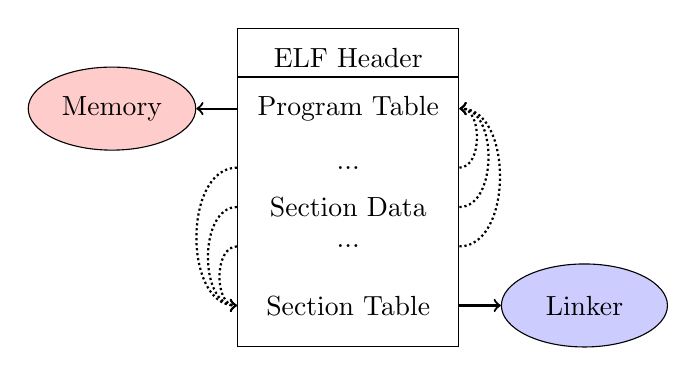
\begin{tikzpicture}
  % ELF File
  \node[draw, rectangle, minimum height=11.5em, minimum width=8em] (whole) at (0,0) {};
  \node[minimum width=8em] (header) at (0,1.65) {ELF Header};
  \draw[thick] (header.south west) -- (header.south east);
  \node[minimum width=8em] (st) at (0,1) {Program Table};
  \node[minimum width=8em] (body1) at (0,0.25) {...};
  \node[minimum width=8em] (body2) at (0,-0.25) {Section Data};
  \node[minimum width=8em] (body3) at (0,-0.75) {...};
  \node[minimum width=8em] (pt) at (0,-1.5) {Section Table};
  % External Users
  \node[draw, ellipse, fill=blue!20, minimum height=3em, minimum width=6em] (linker) at (3,-1.5) {Linker};
  \node[draw, ellipse, fill=red!20, minimum height=3em, minimum width=6em]  (memory) at (-3,1) {Memory};
  % Arrows to Users
  \draw[->,thick] (st.west) to (memory.east);
  \draw[->,thick] (pt.east) to (linker.west);
  % Section Table Arrows
  \draw[->,thick,densely dotted,bend right=90] (body1.east) to (st.east);
  \draw[->,thick,densely dotted,bend right=90] (body2.east) to (st.east);
  \draw[->,thick,densely dotted,bend right=90] (body3.east) to (st.east);
  % Program Table Arrows
  \draw[->,thick,densely dotted,bend right=90] (body1.west) to (pt.west);
  \draw[->,thick,densely dotted,bend right=90] (body2.west) to (pt.west);
  \draw[->,thick,densely dotted,bend right=90] (body3.west) to (pt.west);
\end{tikzpicture}
}
\caption{\label{elf}Sections and their uses in an Executable and
  Linking Format (ELF) file.}
\end{figure}

\noindent Although the majority of ELF files include all three of the
elements shown in Figure~\ref{elf}, only the ELF Header is guaranteed
to exist in all cases.  In {\em executable} ELF files the program
table is also required, and similarly, in {\em linkable} files the
section table is required.

We extend previous work that repaired unstripped Intel and ARM
files~\cite{schulte2013embedded}.  The ELF file is modfied by similar
mutation and crossover operations, but in this case \texttt{net-cgi}
does not include key information on which the earlier work relied,
namely the section table and section name string table.  This
information was used to locate the \texttt{.text} section of the ELF
file where program code is normally stored.  The data in the
\texttt{.text} section were then coerced into a linear array of
assembly instructions (the \emph{genome}) on which mutation and
crossover operated.  Our work removes this dependence by
concatenating the data of every section in the program table that has
a loadable ({\tt PT\_LOAD}) type to produce the genome.  The genome
thus includes all
sections whose data are loaded into memory during program execution
including both code and data.

Mutation operations must change program code without corrupting
the structure of the file or breaking the many memory addresses hard coded
into the program (e.g., as destinations for jumps, loads, or stores).
In general, it is impossible to distinguish between an integer literal
and an address in program code and data, so our mutation operations
are designed to preserve operand absolute sizes and offsets within the
ELF program data.  In addition, the preservation of absolute size
ensures that the modified ELF file may directly replace the original
in the firmware image.  These requirements are more easily met on the
MIPS RISC architecture because every argumented assembly instruction
is exactly one word long~\cite{hennessy1982mips}.

The preservation of offsets allows the use of ``Single point
crossover'' to recombine two ELF files.  An offset in the program
is selected, then bytes from one file are taken up to that offset and
bytes from the other file taken after that offset.  This form of
crossover works especially well because all ELF files are {\em
  homologous}, i.e. they will have similar total length and similar
contents at any given offset.  Single point crossover has previously
been shown effective for the evolution of homologous machine
code~\cite{nordin199912}.  The mutation and crossover operations used
to modify stripped MIPS ELF files are shown in
Figure~\ref{mutation-ops}.

\tikzstyle{asmrow} = [rectangle, draw, minimum width=2em, minimum height=1em]
\begin{figure}[htb]
  \centering
\begin{tikzpicture}
  % Mutation
  \foreach \x in {-3.5,-2.5,-0.5,0.5,2.5,3.5}{
    \foreach \y in {-0.8,-0.4,0,0.4,0.8}{
      \node[asmrow,fill=green!40] at (\x,\y) {};
    }
  }
  % Replace
  \node at (-3,1.25) {Replace};
  \node[asmrow,fill=yellow!20] (c-from) at (-3.5,0.4) {};
  \node[asmrow,fill=blue!60] at (-3.5,-0.4) {};
  % replace-after
  \node[asmrow,fill=yellow!20] at (-2.5,0.4) {};
  \node[asmrow,fill=yellow!20] (c-to) at (-2.5,-0.4) {};
  \node[asmrow,fill=green!40]  at (-2.5,-0.8) {};
  % Delete
  \node at (0,1.25) {Delete};
  \node[asmrow,fill=red!40] (d-from) at (-0.5,0) {};
  % delete-after
  \node[asmrow,fill=white] (d-to) at (0.5,0) {\scriptsize{0x0}};
  % Swap
  \node at (3,1.25) {Swap};
  \node[asmrow,fill=yellow!20] (s1-from) at (2.5,0.4) {};
  \node[asmrow,fill=blue!60] (s2-from) at (2.5,-0.4) {};
  % swap-after
  \node[asmrow,fill=blue!60] (s2-to) at (3.5,0.4) {};
  \node[asmrow,fill=yellow!20] (s1-to) at (3.5,-0.4) {};
  % arrows
  \draw[->,thick] (c-from.east) to (c-to.west);
  \draw[->,thick] (d-from.east) to (d-to.west);
  \draw[->,thick] (s1-from.east) to (s1-to.west);
  \draw[->,thick] (s2-from.east) to (s2-to.west);
  % Crossover
  \node at (0,-1.7) {One Point Crossover};
  \foreach \x in {-1.5,1.5}{
    \foreach \y in {-3.8,-3.4,-3,-2.6,-2.2}{
      \node[asmrow,fill=green!40] at (\x,\y) {};
    }
  }
  \foreach \x in {-0.5}{
    \foreach \y in {-3.8,-3.4,-3,-2.6,-2.2}{
      \node[asmrow,fill=blue!60] at (\x,\y) {};
    }
  }
  \draw[->,thick] (-2,-3.2) to (2,-3.2);
  \node[asmrow,fill=blue!60] at (1.5,-3.4) {};
  \node[asmrow,fill=blue!60] at (1.5,-3.8) {};
\end{tikzpicture}
\caption{Mutation and Crossover operations for stripped MIPS ELF files.  The
  program data are represented as a fixed length array of single-word
  sections.  These operators change these sections maintaining length
  and offset in the array.}
  \label{mutation-ops}
\end{figure}

\subsection{Interactive Regression Testing}
\label{interactive-regression}
Our approach to program repair relies on the ability to assess the
validity of any candidate repair.  The program transformations
do not take into account or preserve the semantics of
the program.  They are more likely to create new bugs or
vulnerabilities than they are to repair undesired behavior, and
an evaluation scheme is required to distinguish between these
cases.

Instead of relying on a pre-existing regression test suite, we assume
only that a demonstration of the exploit provides a single available
test.  By mutating programs without the safety net of a regression
test suite, the evolved ``repairs'' often introduce significant
regressions.  However, by applying a strict minimization process after
the primary repair is evolved, these regressions are usually
removed (\S\ref{minimization}).  The minimization reduces the
difference between the evolved repair and the original program to as
few edits as possible using Delta Debugging~\cite{delta}.  The final
phase of the repair algorithm asks the user to identify any
regressions that remain after the Delta Debugging step through
interactive use of the modified binary, e.g. through a web interface.
If any failures are found, the user must manually write a regression
test encoding the steps of the interactive process which led to the
identification of the regression.  For example after interactively
identifying a broken web page, a user would write a regression test
script which first downloads the broken page's URI, then checks for a
successful download and for desired properties in the downloaded file,
such as the presence of required components of the page.  High-level
pseudocode for the repair algorithm is show in
Figure~\ref{lazy-algorithm}.

Our method is thus an interactive repair process in which the
algorithm searches for a patch that passes every available test
(starting with only the exploit), and then minimizes it using Delta
Debugging.  In a third step, the user evaluates its suitability.  If
the repair is accepted, the process terminates. Otherwise, the user
supplies a new regression test that the repair fails (a witness to its
unsuitability) and the process repeats.  In
\S\ref{repair-demonstration} we find that 80\% of our attempts to
repair the NETGEAR WNDR3700 vulnerabilities did not require any
user-written regression tests.

\begin{figure}[htb]
\begin{algorithmic}[1]
\small
\item[{\textbf{Input: }} {Vulnerable Program, $\mathsf{original}$ : $ELF$}]
\item[{\textbf{Input: }} {Exploit Tests, $\mathsf{vulnerabilities}$ : $[ELF \rightarrow Fitness]$}]
\item[{\textbf{Input: }} {Interactive Check, $\mathsf{goodEnough}$ : $ELF \rightarrow [ELF \rightarrow Fitness]$}]
\item[{\textbf{Output: }} {Patched version of Program}]
  \STATE {\bf let} $new \leftarrow \mathsf{null}$
  \STATE {\bf let} $fitness \leftarrow \mathsf{null}$
  \STATE {\bf let} $suite \leftarrow \mathsf{vulnerabilities}$
  \REPEAT {
    \STATE {\bf let} $\mathsf{full} \leftarrow \mathsf{evolutionarySubroutine}(\mathsf{original}, \mathsf{suite})$
    \STATE $new \leftarrow \mathsf{minimize()}$
    \STATE {\bf let} $newRegressionTests \leftarrow \mathsf{goodEnough}(\mathsf{new})$
    \STATE $\mathsf{suite} \leftarrow \mathsf{suite} ++ \mathsf{newRegressionTests}$
  }
  \UNTIL { $length(\mathsf{newRegressionTests}) \equiv 0$ }
  \RETURN { $\mathsf{new}$ }
\end{algorithmic}
\caption{\label{lazy-algorithm}High-level Pseudocode for interactive
  evolutionary repair algorithm.}
\end{figure}

The \texttt{evolutionarySubroutine} in Figure \ref{lazy-algorithm} is
organized similarly to previous work~\cite{genprog-tse-journal}, but
it uses a \emph{steady state} evolutionary computational
algorithm~\cite{Luke2013Metaheuristics} for reduced memory usage, ease
of parallelization of fitness evaluation, and recognizes the nearness
of the original program to likely valid
repairs~\cite[\S2.2.2]{schulte2014dissertation}.  Figure
\ref{evolutionary-subroutine} gives the high-level pseudocode.

\begin{figure}[htb]
\begin{algorithmic}[1]
\small
\item[{\textbf{Input: }} {Vulnerable Program, $\mathsf{original}$ : $ELF$}]
\item[{\textbf{Input: }} {Test Suite, $\mathsf{suite}$ : $[ELF \rightarrow Fitness]$}]
\item[{\textbf{Parameters: }} {$populationSize$, $tournamentSize$, $crossRate$}]
\item[{\textbf{Output: }} {Patched version of Program}]
  \STATE {\bf let} $fitness \leftarrow \mathsf{evaluate}(\mathsf{original}, \mathsf{suite})$
  \STATE {\bf let} $pop \leftarrow \mathsf{populationSize}$ copies of $\langle \mathsf{original}, \mathsf{fitness} \rangle$
  \REPEAT {
    \IF {$\mathsf{Random}() < CrossRate$}
      \STATE {\bf let} $\mathsf{p_{1}} \leftarrow \mathsf{tournament}(\mathsf{pop}, \mathsf{tounamentSize}, +)$
      \STATE {\bf let} $\mathsf{p_{2}} \leftarrow \mathsf{tournament}(\mathsf{pop}, \mathsf{tounamentSize}, +)$
      \STATE {\bf let} $\mathsf{p} \leftarrow \mathsf{crossover}(\mathsf{p_{1}}, \mathsf{p_{2}})$
    \ELSE
      \STATE $p \leftarrow \mathsf{tournament}(\mathsf{pop}, \mathsf{tounamentSize}, +)$
    \ENDIF
    \STATE {\bf let} $p' \leftarrow \mathsf{Mutate}(p)$
    \STATE {\bf let} $fitness \leftarrow \mathsf{evaluate}(\mathsf{suite}, \mathsf{p'})$
    \STATE $\mathsf{incorporate}(pop,\langle p', \mathsf{Fitness}(\mathsf{Run}(p')) \rangle)$
    \IF {$\mathsf{length}(\mathsf{pop}) > \mathsf{maxPopulationSize}$}
      \STATE $\mathsf{evict}(\mathsf{pop}, \mathsf{tournament}(\mathsf{pop}, \mathsf{tounamentSize}, -))$
    \ENDIF
  }
  \UNTIL { $\mathsf{fitness} > \mathsf{length}(\mathsf{suite})$ }
  \RETURN { $\mathsf{p'}$ }
\end{algorithmic}
\caption{\label{evolutionary-subroutine}High-level Pseudocode for the
  steady state parallel evolutionary repair subroutine.}
\end{figure}

\noindent Note that every time the user rejects the solution returned
by \texttt{evolutionarySubroutine}, the evolved and minimized solution
is discarded and a new population is generated by recopying the
original in \texttt{evolutionarySubroutine}.  Most applications of EC
begin with a randomly generated population, but we begin with a
population of copies of the original.  This is because the original
program is in fact a highly engineered solution to the program fitness
landscape and likely to lay close to acceptable repairs.  This
algorithmic choice acknowledges the fitness of the original program,
and for this reason gives it primacy over the evolved solutions of
previous iterations (which may well have evolved into fitness valleys
as in run 8 Table \ref{minimized-stats}).

\section{Repairing the NETGEAR Vulnerabilities}
\label{repair-demonstration}

We first describe the experimental setup used to test the repair
technique on the NETGEAR WNDR3700 exploit (\S\ref{methodology}).  We
then analyze the results of ten repair attempts (\S\ref{analysis}).

\subsection{Methodology}
\label{methodology}
All repairs were performed on a server-class machine with 32 physical
Intel Xeon 2.60GHz cores, Hyper-Threading and 120 GB of Memory. We
used a test harness to assess the fitness of each program variant
(\S\ref{fitness-evaluation}) and report parameters used in the
experiments (\S\ref{sec:parameters}).

\subsubsection{Fitness Evaluation}
\label{fitness-evaluation}
We used 32 QEMU virtual machines, each
running Debian Linux with the NETGEAR router firmware environment
available inside of a \texttt{chroot}.  The repair algorithm
uses 32 threads for parallel fitness evaluation.  Each thread is
paired with a single QEMU VM on which it tests fitness.

The test framework includes both a host and a guest test script.  The
host script runs on the server performing repair and the guest script
runs in a MIPS virtual machine.  The host script copies a
variant of the \texttt{net-cgi} executable to the guest VM where the
guest test script executes \texttt{net-cgi} the command line and
reports a result of {\sc Pass}, {\sc Fail}, or {\sc Error} for each
test.  These values are then used to calculate the variant's scalar
fitness.

{\sc Pass} indicates that the program completed successfully and
produced the correct result, {\sc Fail} indicates that the program
completed successfully but produced an incorrect result, and {\sc
  Error} indicates that the program execution did not complete
successfully due to early termination (e.g., because of a segfault) or
by a non-zero ``errno'' exit value.

\subsubsection{Repair Parameters}
\label{sec:parameters}
Our algorithm uses the following parameters.  The maximum population size is
512 individuals, selection is performed using a tournament size of
two.  When the population overflows the maximum population size, an
individual is selected for eviction using tournament selection in
reverse.  Newly generated individuals undergo crossover two-thirds of
the time.

These parameters differ significantly from those used in previous
evolutionary computation (EC) repair algorithms
(e.g.,~\cite{forrest2009genetic,legoues2011systematicstudy,le2012representations}).
Specifically, we use larger populations (512 instead of 40
individuals), running for many more fitness evaluations ($\leq$100,000
instead of $\leq$400).  The parameters used here are in line with
those used in other EC publications given the size of the
\texttt{net-cgi} binary, and they help compensate for the lack of
fault localization information.

The increased memory required by the larger population size is offset
by the use of a steady-state~\cite{Luke2013Metaheuristics} EC
algorithm, and the increased computational demand of the greater
number of fitness evaluations is offset by parallelization of fitness
evaluation.

\subsection{Experimental Results}
\label{analysis}

We report results for the time typically taken to generate a repair
(\S\ref{runtime}), the effect of eliminating fault localization
(\S\ref{no-fault-localization}), and the impact of the minimization
process (\S\ref{minimization}), both with respect to the size of the
repair in terms of byte difference from the original and in terms of
the fitness improvement.  Finally we demonstrate how multiple repairs
can be discovered iteratively by the repair process
(\S\ref{iterative-repair}).

\subsubsection{Repair Runtime}
\label{runtime}
In 8 of the 10 runs of the algorithm (with random restarts), the three
exploit tests alone were sufficient to generate a satisfactory repair
(determined using a withheld regression test suite hand-written by the
authors\footnote{\url{https://github.com/eschulte/netgear-repair/blob/master/bin/test-cgi}}),
and the third phase of user-generated tests was not required.

In these cases the repair process took an average of ~36,000 total
fitness evaluations requiring on average 86.6 minutes to find a repair
using 32 virtual machines for parallelized fitness evaluation.

\subsubsection{Repair without Fault Localization}
\label{no-fault-localization}

In the NETGEAR scenario, we do not have access to fault localization
information.  Although commonly required, fault localization
information may sometimes {\em over-constrain} the search operators
(mutation and crossover) \cite{schulte2013optimization}, preventing
the discovery of valid repairs.

\begin{figure}[htb]
  \centering
  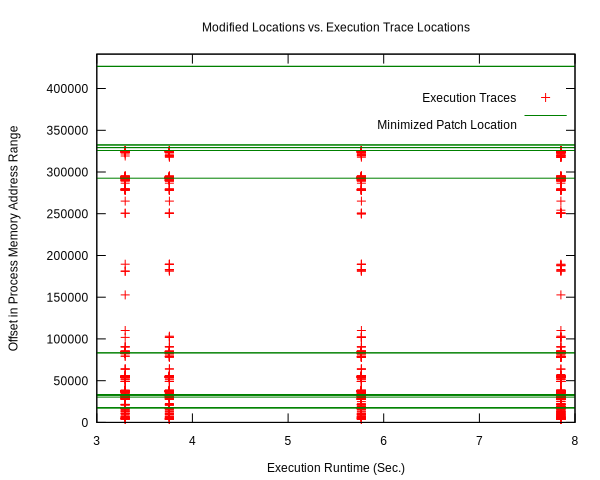
\includegraphics[width=0.46\textwidth]{figures/ts-cov-and-runtime-w-min.pdf}
  \caption{Code modifications occur in different locations from
    execution traces: The location of every edit in a minimized
    successful repair is plotted as a horizontal line.  Only 2 of the
    22 minimized edit locations are within 3 bytes of a sample from
    any test suite execution.  Each vertical column shows points of
    execution traces from one test suite.  Test suites shown from left
    to right are 3 tests (exploit tests only), 4, 7, and 11 tests (all
    exploit and author-generated regression tests), with 330, 399,
    518, and 596 sampled execution locations respectively.}
  \label{ts-cov-rt-w-min}
\end{figure}

One of the NETGEAR vulnerabilities exemplifies this issue.  As shown
in Figure \ref{ts-cov-rt-w-min}, fault localization might have
prevented the repair process from succeeding.  The figure shows that
many of the program edit locations for successful repairs were not
visited by the execution trace.  In fact, only 2 of these 22 program
edit locations were within 3 instructions of the execution traces.  In
fact, one of the edit locations was in the {\tt .rodata} section of
the binary which could never appear in an execution trace.  The {\tt
  .rodata} section typically holds read-only data such as static
variables. Such non-code sections of the executable were only mutated
because of the lack of section names as discussed in
\S\ref{mutate-mips}.  This surprising result suggests that earlier
work, which confines edit operations to execution traces, would
possibly be unable to repair the NETGEAR bugs. Testing this
possibility more definitively would require developer-written
regression tests, however. While fault localization is reasonable for
source-level repairs (e.g., by definition the defect must be
addressable in a visited statement), at the binary level repair can
often be created by changing data~\cite{demsky06-tse,clearview}. While
fault localization does reduce the search time, for binary-level
repairs it may cause a larger number of viable repair candidates to be
excluded from the search space.

\subsubsection{The impact of Minimization}
\label{minimization}

In some cases the initial suggested repair, known as the
\emph{primary} repair, was not satisfactory.  For
example, suggested repairs sometimes worked when \texttt{net-cgi} was
called directly on the command line but not through the embedded
$\mu$HTTPd webserver,\footnote{\url{http://wiki.openwrt.org/doc/uci/uhttpd}}
or the repaired file failed to serve pages not used in the
exploit test.  However, Table \ref{minimized-stats} shows that in most
cases the minimized version of the repair was satisfactory,
successfully passing all hand-written regression tests, even those not used
during the repair process.

\begin{table}[htb]
\centering
\adjustbox{width=0.5\textwidth}{
\begin{tabular}{rrrrrr}
Run  & Fit Evals & Full Diff & Min Diff & Full Fit & Min Fit \\
\toprule
0    & 90405     & 500       & 2        & 8        & 22      \\
1    & 17231     & 134       & 3        & 22       & 22      \\
2    & 26879     & 205       & 2        & 21       & 22      \\
3    & 23764     & 199       & 2        & 19       & 22      \\
4    & 47906     & 319       & 2        & 6        & 6       \\
5    & 13102     & 95        & 2        & 16       & 22      \\
6    & 76960     & 556       & 3        & 17       & 22      \\
7    & 11831     & 79        & 3        & 20       & 22      \\
8    & 2846      & 10        & 1        & 14       & 14      \\
9    & 25600     & 182       & 2        & 21       & 22      \\
\bottomrule
mean & 33652.4   & 227.9     & 2.2      & 16.4     & 19.6    \\
\end{tabular}
}
\caption{\label{minimized-stats}The
evolved repair before and after minimization.  In these columns ``Full''
refers to evolved solutions before minimization and ``Min'' refers to
solutions after.  Columns labeled ``Diff'' report the number
of unified diff windows against the original program data. The columns
labeled ``Fit'' report fitness as measured with a full regression test
suite, including the exploit tests.  The maximum possible fitness
score is 22, indicating a successful repair.}
\end{table}

As shown in Table \ref{minimized-stats}, the initial evolved repair
differed from the original at over 200 locations on average in the ELF
program data, while the minimized repairs differed at only 1--3
locations on average.  This great discrepancy is due to the
accumulation of candidate edits in non-tested portions of the program
data.  Since these portions of the program were not tested, there was
no evolutionary pressure to purge the harmful edits.
Delta Debugging eliminates these edits.

Given the small number of edits which remain after minimization it is
possible that, at least for those repairs which minimize to two diff
windows (Column ``Min Diff'' in Table \ref{minimized-stats})
corresponding to the two vulnerabilities in the original program, the
use of a systematic exhaustive search that {\em only} retains program
edits that strictly improve fitness may be sufficient to perform
program repair.

\subsubsection{Iterative Repair}
\label{iterative-repair}
The NETGEAR repairs required two distinct modifications, addressing
two different vulnerabilities in a single evolutionary run.  This is
an instance of ``iterative repair'' of multiple vulnerabilities which
has not previously been demonstrated in real-world software.

\section{Related Work}
\label{sec:related-work}

Evolutionary computation (EC) refers to the use of natural selection
as a search heuristic~\cite{holland1992adaptation,koza1992genetic}.
EC techniques have been developed to operate directly on machine
code~\cite{kuhling2002brute}, and more recently they have been applied
to the problem of software source-code
repair~\cite{genprog-tse-journal,arcuri2011evolutionary},
optimization~\cite{sitthi2011genetic,schulte2013optimization,LangdonAndHarmon2015a},
to repairing assembly code and binary ELF
files~\cite{SchulteEtAl2010a,schulte2013embedded}, to combine
different versions of software~\cite{foster2010object,petke2014using},
and to the incorporation of new functionality into existing
software~\cite{harman2014babel}.  Software is inherently robust to
mutation, a property termed {\em software mutational
  robustness}~\cite{schulte2013software}.  Software mutational
robustness has been measured in software represented using source
code, intermediate representations (e.g., {\sc Cil}, LLVM IR),
assembly code, and binary executables~\cite{schulte2014dissertation}.

In addition to the EC methods mentioned above, Clearview
\cite{clearview} automatically patches errors in running binaries by
learning invariants of running executables, and then reacting to
attacks or bugs that invalidate the invariants by applying predefined
patches.

\section{Discussion}
\label{sec:discussion}

The results presented here open up the possibility that end users
could repair software vulnerabilities in closed source software
without special information or aid from the software vendor.

\subsection{Threats to Validity}

There are several caveats associated with this initial work.  First,
we demonstrated repair on a single executable, and it is possible that
our success in the absence of regression test suite will not
generalize.  However, our results do not appear to be based on any
property unique to the NETGEAR vulnerabilities.  We conjecture that
our success at finding functional repairs is due to
the beneficial impact of minimization and to \emph{software mutational
  robustness}~\cite{schulte2013software,schulte2014dissertation}.

We demonstrated our repairs running in a virtualized environment and
not natively in the router.  Although we did not test our repairs on
physical NETGEAR WNDR3700 hardware, we are confident that our repairs
would have the same effect on hardware as they do in emulation, given
that they affect aspects of program logic not directly related to the
execution environment.

\subsection{Future Work}

Although security vulnerabilities are serious, an important
implication of this technique is the ability of end users to change
non-security aspects of software, i.e. the {\em customization} of COTS
binaries by end users.  This approach could be applied to {\em any}
feature of program behavior which may be encoded in a fitness
function.  Although the direct synthesis of novel program behavior is
certainly a more challenging task than the patching of
vulnerabilities, there are many plausible and desirable yet simple
software customizations, even including the direct removal of unwanted
software features.

This technique could be combined with an automated testing or exploit
generation technique, such as fuzz testing~\cite{miller1990empirical},
to automatically ``harden'' closed source applications.  Such a
process would allow end users to proactively protect their devices
from a wide range of easily generated attacks and could potentially be
used to disrupt the large mono-culture of commercial
firmware~\cite{ieee-sp-09}.  The technique could also be adapted by
users to disable or break undesirable or insecure functionality (e.g.,
password reset) in closed-source applications.  Finally, the technique
could be distributed across multiple untrusted peers and used to
distribute self-certifying
patches~\cite{costa2008vigilante,schulte2013embedded}.

Whenever a patch is distributed there is the risk that a malicious
individual will reverse-engineering an exploit from the patch
text~\cite{brumley2008automatic}.  As shown in Table
\ref{minimized-stats} our technique can generate edits that are not
directly relevant to the repaired exploit.  It may be possible to
leverage these harmless, i.e. {\em neutral}, edits to reduce the risk
of reverse engineering.  By skipping the post-evolutionary
minimization step, these irrelevant edits would be retained resulting
in obfuscated patches which hide the relevant edits.  However,
skipping minimization would likely require a regression test suite or
other method of ensuring semantic correctness.

\section{Conclusion}

The paper described a method that enables end users to repair COTS
software without cooperation from the software vendor.  This is
accomplished through a number of novel extension to existing
techniques of evolutionary program repair, including the use of user
interaction and removing the requirements of a regression test suite
and fault localization.  We demonstrate the method by repairing two
security vulnerabilities in the popular NETGEAR WNDR3700 router,
vulnerabilities that currently exist in many actively used devices and
to the authors knowledge have not been addressed by NETGEAR.

\section{Acknowledgments}
\label{sec-7}
We thank Z. Cutlip, who analyzed and announced the NETGEAR
vulnerabilities and helped us reproduce the vulnerabilities locally;
we thank M. Harmon, for discussions of automated program repair
without a regression test suite; and S. Harding for suggesting the
interactive regression repair algorithm.  Partial support of this work
provided by NSF (SHF-0905236), DARPA (FA8750-15-C-0118), AFRL
(FA8750-15-2-0075), DHS (HSHQDC-14-C-00055), and the Santa Fe
Institute.  Any opinions, findings and conclusions or recommendations
expressed in this material are those of the authors and do not
necessarily reflect the views of the supporting agencies.

\bibliographystyle{plain}
\small
\bibliography{netgear-repair}

\end{document}
